\documentclass{article}
\usepackage[utf8]{inputenc}
\usepackage[a4paper, total={6in, 8in}]{geometry}

\usepackage{algorithm}
\usepackage{algpseudocode}
\usepackage{amsmath}
\newcommand\ddfrac[2]{\frac{\displaystyle #1}{\displaystyle #2}}
\usepackage{graphicx}
\usepackage[dvipsnames]{xcolor}
\usepackage[colorlinks=true,urlcolor=Blue,linkcolor=Blue,citecolor=Blue]{hyperref}

\title{INFO-H410 Project}
\author{PARDON Mathieu, DIAZ Y SUAREZ Esteban, WAFFLARD Guillaume}
\date{}

% Content of report:
%   - The content of your project
%   - The theory and AI algorithms underlying it
%   - Some snapshots of your running code.

\begin{document}

\maketitle
\tableofcontents
\clearpage


\section{Introduction}

This report will give a description of the implementation and the theoretical aspects used for the project of the course INFO-H410: Techniques of AI. Our project consists in the development of an artificial intelligence for the game Othello\copyright. In this game, two players play against each other on an 8×8 square board. The board contains initially 2 pieces of each color (black and white) disposed alternatively in the center of the board. Players take turns placing a piece of their own color on the board (the spaces where pieces can be placed must meet certain constraints) and thus all pieces of the opponent's color that are between two pieces of the player's color are converted into the player's color. The game ends when the board is completely filled with pieces or when neither player has any more moves available. The player with the most pieces of his color on the board wins the game. In order to compare several artificial intelligence methods on this game, we developed a machine learning algorithm and a search algorithm. Machine learning agents have been trained with different hyper-parameters and all types of agents have been tested against each other.

\section{Software architecture}

\subsection{Graphical interface}

The directory \textit{gui} contains classes that implements the graphical user interface. The graphical interface has been developed with the library \textit{PyQt5}. The class \textit{ManagerUI} performs some initializations and manages the navigation between menus. The class \textit{MenuTab} displays the main menu. The class \textit{GameTab} offers an interface to display a match between two agents and manages the user inputs if one of the agents is human. The class \textit{WindowUtils} implements some repetitive UI-related initializations and is inherited by two previous classes.

\subsection{Game implementation}

The directory \textit{game} contains files related to the game management. The class \textit{OthelloGame} represents an instance of the game. It contains an attribute of type list representing the 64 cases of the board of the game. Elements of the list can be None if it represents an empty case, True if it contains a white piece and False if it contains a black piece. The class implements several methods in relation to the game rules, for example: check if a move can be played by a player, apply the move of a player, return all playable moves for a given player... The class \textit{GameManager} contains an instance of \textit{OthelloGame} and uses its methods to supervise the course of the game: initializes classes of agents that will play the game, call their method \textit{make\_move} alternatively and updates the board each turn. In the case of a match, it communicates with the user interface to display the progression of the match. If one of the agents is a human player, it also communicates with the UI to receive user input (and indicate whether the input is valid with regard to the game rules). In the case of training a machine learning agent or comparison between two agents, \textit{GameManager} restarts the game the required number of times and send the progression (in percent) to the interface.

Finally, the abstract class \textit{Player} is inherited by classes that represent different types of agents. It contains an abstract method \textit{make\_move} which is the generic name that will be used by \textit{GameManager} to request a move to an agent (NB: in the case of the \textit{PlayerHuman} class, this method is only defined for compatibility as a human move is concretely performed by the user interface).

\subsection{Storage}

The file \textit{NNstorage} of the \textit{db} directory provides some methods to store and retrieve data related to machine learning agents such as the weight matrices, the activation function and the learning strategy used to train them. A method to initialize a new neural network is also defined.

\subsection{Artificial intelligence agents}

Finally, the directory \textit{ai} defines three classes inheriting class \textit{Player} described above that represents the agents that can play the game. The algorithms used will be described in details in the following sections but here is an overview of their composition in terms of software:

\begin{itemize}
    \item \textit{PlayerRandom} defines one single method that consists of returning one move randomly. Mainly used for debugging and testing whether other (real) ai agents perform at least better than a random agent.
    \item \textit{PlayerML} defines the methods to train a neural network (back propagation) and use it to estimate the probability of victory of a given game state (forward pass).
    \item \textit{PlayerMinimax} try to determine the best move with a search algorithm.
\end{itemize}

\subsection{Software and external libraries}

The game has been developed with the following tools:

\begin{itemize}
    \item Python version 3.8.10
    \item User interface library PyQt5 version 5.12.8
    \item Scientific computing library NumPy version 1.21.1
\end{itemize}

\section{Machine learning agent}

\subsection{Structure of the network}

\subsubsection{Game state encoding}

For the neural networks operations, a game state is represented with one-hot encoding on a numpy array of size 128: the 64 first elements represent the position of black pieces on the board and the last 64 bits represent the position of the white pieces, an element is 1 if a piece of the corresponding color is present on the given position and 0 otherwise (of course, any two elements of this array separated by 64 indices cannot be 1 simultaneously). The board is considered line-wise, from left to right and from top to bottom.

\subsubsection{Prediction using the neural network}

The machine learning agent uses a neural network made up of three layers: input layer, one hidden layer and output layer. According to the representation of a game state, the input layer of the network is made up of 128 neurons. The model is used to return an estimation of the victory probability given an input game state, so the output layer is made up of 1 single neuron. The hidden layer has been tested with different sizes ranging from 20 to 100 neurons (details in Benchmark section). The weights of the network are randomly initialized with a normal distribution of mean $0$ and standard deviation $0.0001$. Here are the \hyperref[alg:fp-pseudo]{pseudocode} and the \hyperref[code:fp-code]{implementation} of the forward pass algorithm that is used to get an estimation of the victory probability of an input state using the network.

\begin{algorithm}[H]
	\caption{Forward pass algorithm pseudocode}
    \label{alg:fp-pseudo}
	\begin{algorithmic}[1]
		\For {each neuron $i$ of intermediate layer}
		    \State $X_{i}^{(int)} \leftarrow \sum_{j}{W_{ij} X_{j}^{(inp)}}$
		    \State $P_{i}^{(int)} \leftarrow f(X_{i}^{(int)})$
		\EndFor
		\State $x^{(out)} \leftarrow \sum_{i}{W_{i}^{(out)}P_ {i}^{(int)}}$
		\State $p^{(out)} \leftarrow f(x^{(out)})$
	\end{algorithmic}
\end{algorithm}

\underline{Notations}: $X^{(inp)}$ represents the input layer, $W^{(int)}$ and $W^{(out)}$ refer to the weight matrices of the network (between the input layer and the intermediate layer and between the intermediate layer and the output layer respectively). The quantity $X_{i}^{(int)}$ is the value of the $i^{th}$ neuron of the intermediate layer and $P_{i}^{(int)}$ is the value at the output of that same neuron, obtained passing the value of the neuron as argument of the chosen activation function $f$. $x^{(out)}$ and $p^{(out)}$ are the same quantities for the output neuron.

\begin{figure}[H]
    \begin{center}
      \label{code:fp-code}
      \makebox[\textwidth]{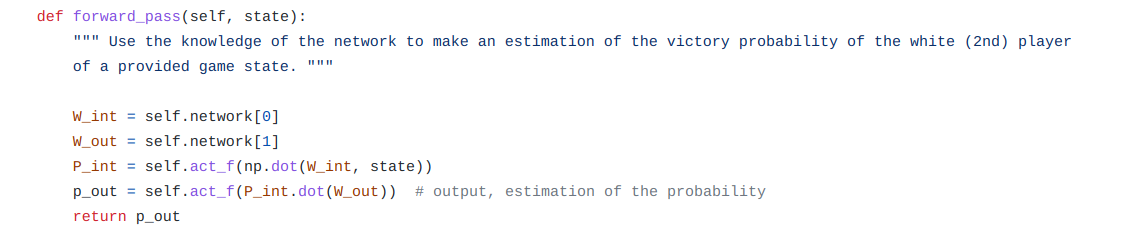
\includegraphics[width=\paperwidth]{forward_pass_code.png}}
      \caption{Implementation of the forward pass algorithm}
    \end{center}
\end{figure}

\subsubsection{Black and white player perspectives}

 To speed up the learning procedure and be able to use the same network to make predictions both as white and black, predictions will be considered as being from the point of view of white. Therefore, if the agent has to make a choice as black player, it will consider the complement of the probability estimations for the moves it can play. Indeed, taking the move with the smallest probability is in fact reducing the victory probability of the white player and therefore maximizing its.

\subsection{Learning strategies}

\subsubsection{Q-learning}

The first learning strategy used to train the neural network is Q-learning. At each turn, the difference ($\delta$) between the probability estimation of the actual state and the probability estimation of the most promising possible next state is computed. This value serves as the basis for the update of the network weights. The weights are updated with a \textit{backpropagation} algorithm. See the \hyperref[alg:backprop]{pseudocode} here, and the \hyperref[code:bp-code]{implementation} here.

\begin{algorithm}[H]
	\caption{Backpropagation for Q-learnign algorithm}
	\label{alg:backprop}
	\begin{algorithmic}[1]
	    \State $\delta \leftarrow p^{(out)}(s',W^{(int)},W^{(out)})-p^{(out)}(s*,W^{(int)},W^{(out)}) $
		\For {each neuron $i$ of intermediate layer}
		    \State $\Delta_{i}^{(int)} \leftarrow grad^{(out)} \cdot W_{i}^{(out)} \cdot grad_{i}^{(int)}$
    		\For {each neuron $j$ of input layer}
    		    \State $ W_{ij}^{(int)} \leftarrow W_{ij}^{(int)} - \alpha \cdot \delta \cdot \Delta_{i}^{(int)} \cdot X_{j} $
	    	\EndFor
	    	\State $ W_{i}^{(out)} \leftarrow W_{i}^{(out)} - \alpha \cdot \delta \cdot grad^{(out)} \cdot P_{i}^{(int)} $
	    \EndFor
	\end{algorithmic} 
\end{algorithm}

\underline{Notations}: $s'$ is the current state, $grad$ is the derivative of the activation function and $s*$ is the state that the neural network evaluates as most promising for a given player.

\begin{figure}[H]
    \begin{center}
      \label{code:bp-code}
      \makebox[\textwidth]{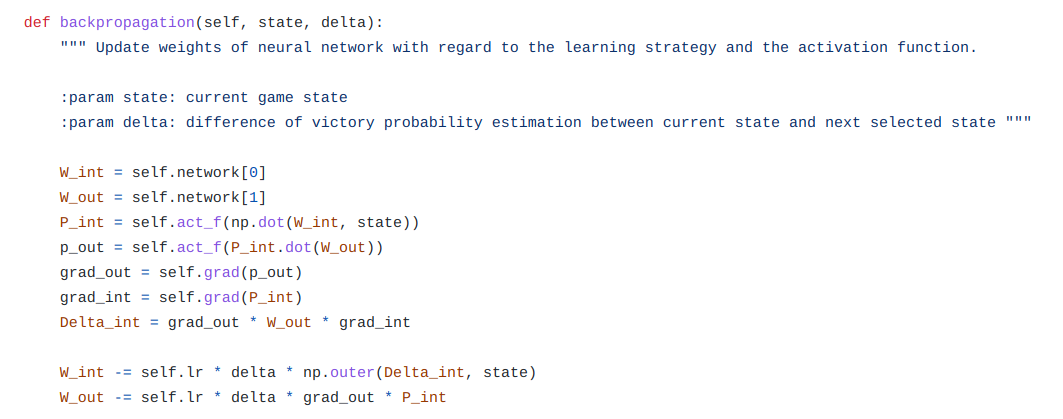
\includegraphics[width=\paperwidth]{backpropagation_code.png}}
      \caption{Implementation of the backpropagation algorithm}
    \end{center}
\end{figure}

\underline{Notations}: $self.grad$ refers to the derivative of the activation function.

\subsubsection{SARSA}

The SARSA learning rule is very similar to the Q-learning rule. The only difference is the state to which the current state is compared: in Q-learning, the comparison was made with the most promising state (independently of the choice made that turn) whereas in SARSA, the comparison is made with the state chosen at that turn.

\subsection{Activation functions}

Here are the different activation functions and their derivative considered in this project.

\begin{itemize}
    \item Sigmoïd
\end{itemize}

$$ \sigma(x) =  \frac{1}{1 + e^{-x}}  $$ 
$$ \sigma'(x) =  \sigma(x)(1 - \sigma(x))  $$ 

\begin{itemize}
    \item ReLU
\end{itemize}

$$ f(x) =  max(0, x)  $$ 
\[
    f'(x)= 
\begin{cases}
    1,         & \text{if } x > 0\\
    0,         & \text{if } x < 0\\
    undefined & \text{if } x = 0
\end{cases}
\]

The value of the derivative is unedefined in $0$ as ReLU is non-differentiable in $0$. In this project, it will be arbitrarily set to 0 to avoid having to deal with undefined values and as this is the choice made by \href{https://hal.archives-ouvertes.fr/hal-03265059v2/document\#:~:text=The\%20value\%20of\%20the\%20derivative,the\%20subgradient\%20from\%20convex\%20analysis}{PyTorch and TensorFlow}.

\begin{itemize}
    \item Hyperbolic Tangent
\end{itemize}

$$ tanh(x) =  \frac{e^{x} - e^{-x}}{e^{x} + e^{-x}}  $$ 
$$ tanh'(x) = \frac{1}{cosh^{2}(x)}  $$ 

\subsection{Move selection rules}

\begin{itemize}
    \item Epsilon-greedy
\end{itemize}

The epsilon-greedy strategy depends on a parameter $\epsilon \in [0, 1]$. It will take the most promising move with a probability $1 - \epsilon$ and a random move (possibly the most promising) in other cases.

\begin{itemize}
    \item Softmax-exponential
\end{itemize}

The softmax-exponential strategy will always take a move randomly. The possible moves will be attributed a probability given by a softmax-exponential distribution and depending on their winning probability estimation. Let $S$ be the set of states that the agent can reach by mean of its available moves and $s$ one of these states having a probability estimation of $p_{s}$. This state will be attributed the probability: $\ddfrac{e^{p_{s}}}{\sum_{t \in S}{e^{p_{t}}}}$.

\section{Minimax agent}
The MiniMax algorithm is Depth-First Search recursive algorithm. It can be seen as tree where each node is a state.
The root node is the current state and the child of a node is a state that can be reached after one move, from the parent state.
Considering that each player will the move in its higher interest, the algorithm imagine that the player must player its best move, knowing the its opponent will always its worst move.

...

At each node is associated a value, which is the estimation of the value of the move

...

the importance of the parameter depth

The complexity of this algorithm is exponential : 0($b^m$) that is the number of possible move for each state to the power of the depth of the tree.
It is obvious that the more futures moves are considered, the better will be the result, but also the more will be the computational power.

Prunning...

Our Minimax player has good result against human. The comparaison of performance will be described in the Benchmark section\ref{sec:benchmark}.
Until depth = 3, the player select a move under the second.
For depth = 4 to 5, it may take a few seconds to choose a move, especially when the number of possible moves is high.
For depth = 6 and more, it takes at least 5 seconds, which is slow even for a human player.

\subsection{Heursitic}
The minimax algorithm depends on an heuristic. Indeed, it need to evaluate how much a move is interesting for him %him or it ?
or not. This evaluation is given by an heuristic, that is based on human strategies.
The heuristic return a value that depends on all these rules :
\begin{itemize}
    \item rule 1
    \item rule 2
\end{itemize}
The weight of each rule is a parameter that can be modified to improve the result. Obviously, the rules "the player win" and "the other player win", are weighted respectively
to \textit{infinity} and $-$\textit{infinity}.
 -faire test pour évaluer meilleure heuristique


\section{Benchmark} \label{sec:benchmark}

\section{Conclusion}

\end{document}
